\documentclass{standalone}
\usepackage{tikz}

\begin{document}
 	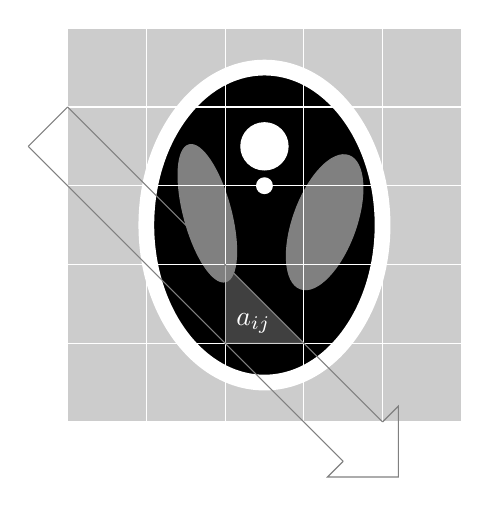
\begin{tikzpicture}
 		\draw[fill=black](0,0)--(5,0)--(5,5)--(5,0)--(0,0);
 		\draw[ fill=black!20!white]  (0,0) grid (5,5) rectangle (0,0);
 		\draw[white,fill=black,line width=0.2cm] (2.5,2.5) ellipse (1.5cm and 2cm);
 		\draw[gray,fill=gray,rotate=15] (2.4,2.1) ellipse (0.3cm and 0.9cm);
 		\draw[gray,fill=gray,rotate=-20] (2.2,3.5) ellipse (0.4cm and 0.9cm);
 		\draw[white,fill=white](2.5,3.5) circle (0.3 cm);
 		\draw[white,fill=white](2.5,3) circle (0.1 cm);
 		\draw[white] (0,0) grid (5,5) ;
 		\draw[gray, name=above] (4,0) -- (0,4);
  		\draw[gray, name=below] (3.5,-0.5) -- (-0.5,3.5);
  		\draw[gray, fill=gray, opacity=0.5] (2,2) -- (3,1) -- (2,1) -- (2,1);
  		\draw[gray] (4,0)--(4.2,0.2)--(4.2,-0.7)--(3.3,-0.7)-- (3.5,-0.5);
  		\draw[gray] (-0.5,3.5)-- (0,4);
  		\node[white,below left] at (2.7,1.5) {$a_{ij}$};
 	\end{tikzpicture}
\end{document}
